% !TeX root = Protokoll.tex


\section{Magnetische Momente}
Ein Elektron im Atom besitzt zu einem den Bahndrehimpuls $\vec{l}$ und zum anderen wie ein Eigendrehimpuls fungierenden Spin $\vec{s}$.
Die Beträge dieser vektoriellen Größen werden bestimmt durch
\begin{align}
	|\vec{l}|=&\sqrt{l(l+1)}\hbar\\
	\nonumber &\text{und}\\
	|\vec{s}|=&\sqrt{s(s+1)}\hbar.
\end{align}
Dabei sind $l$ und $s$ die Quantenzahlen, sowie $\hbar$ das Plancksche Wirkungsquantum.
Aufgrund der Ladung der Elektronen, entsteht da durch magnetische Momente $\vec{\mu_l}$ und $\vec{\mu_s}$ .
Mithilfe des Bohrschen Magnetons 
\begin{align}
	\mu_B:=-\frac{1}{2}e_0 \frac{\hbar}{m_0},
\end{align}
lassen sich diese Momente berechnen durch
\begin{align}
	\vec{\mu}_l=&-\mu_B\sqrt{l(l+1)}\vec{e}_l\\
	\nonumber &\text{und}\\
	\vec{\mu}_s=&-g_s\,\mu_B\sqrt{s(s+1)}\vec{e}_s.
\end{align}
Hier sind ist $e_0$ die Elementarladung, $m_0$ die Elektronmasse.
Weiter wird für $\vec{\mu}_s$ der Landé-Faktor eingeführt, der die Stärke der der Kopplung des Spins ans magnetische Moment beschreibt.\\
Für Atome mit mehr als ein Elektron gibt es verschiedene Arten, wie der Bahndrehimpulse und der Spin wechselwirken können.
Grundlegend werde zwei grundlegenden Fälle unterschieden.
Zum einen für Atome mit niedriger Kernladungszahl und zum anderen mit hoher.
Bei Atomen mit kleiner Kernladungszahl, ist die Wechselwirkungen den Drehimpulsen groß.
Deshalb lässt sich ein Gesamtdrehimpuls definieren als
\begin{align}
	\vec{L}:=\sum_i \vec{l}_i\, \text{ mit }\, |\vec{L}|=\sqrt{L(L+1)}\hbar.
\end{align}
Weil der Drehimpuls abgeschlossener Schalen immer Null ist, reicht es über die Drehimpulse der der nicht abgeschlossenen Schalen zu summieren.
Es treten nur Gesamtdrehimpulse auf, deren Quantenzahl ganzzahlig ist.
Dabei werden den Quantenzahlen L=0, 1, 2 oder 3 den Termen S, P, D oder F zugewiesen.\\
Zu dem Gesamtdrehimpuls lässt sich ein magnetisches Moment $\vec{\mu}_L$ aufstellen als
\begin{align}
	|\vec{\mu}_L|=\mu_B\sqrt{L(L+1}).
\end{align}
Es lässt sich weiter ein Gesamtspin $\vec{S}$ definieren als
\begin{align}
	\vec{S}=\sum_is_i \text{ mit } |\vec{S}|=\sqrt{S(S+1)}\hbar.
\end{align}
Für die Gesamtspinquantenzahl gilt $S=\frac{N}{2},\ \frac{N}{2}-1 ,\ \dots,\ \frac{1}{2},\ 0$, wobei $N$ die Anzahl der Elektronen der nicht abgeschlossenen Schale ist.
Das magnetische Moment das durch den Gesamtspin hervorgerufen wird lässt sich mit
\begin{align}
	|\vec{\mu}_S|=g_S\ \mu_B\sqrt{S(S+1)}
\end{align}
berechnen.
Bei nicht zu großen externen Magnetfeldern lässt sich der Gesamtdrehimpuls bestimmen als
\begin{align}
	\vec{J}=\vec{L}+\vec{S} \ \text{ mit }\ |\vec{J}|=\sqrt{J(J+1)}\hbar.
\end{align}
Ein Energie Niveau kann mithilfe von 
\begin{align}
	{}^ML_J
\end{align}
ausgedrückt werden.
Darin Bezeichnet $M=2S+1$ und $L\in\{S,\ P,\ D,\ F\}$ referiert zu der Quantenzahlen des Bahndrehimpulses.
Diese Art der Kopplung wird LS-Kopplung genannt.\\
Der Zweite Fall, der mit Großer Kernladungszahl, wird j-j-Kopplung genannt.
Hier koppelt der Spin und der Bahndrehimpuls eines Elektrons stark, gegenüber der Anteile der anderen Elektronen.


\subsection{Vorbereitungaufgaben}
\newpage
\FloatBarrier
\begin{figure}[!h]
\centering
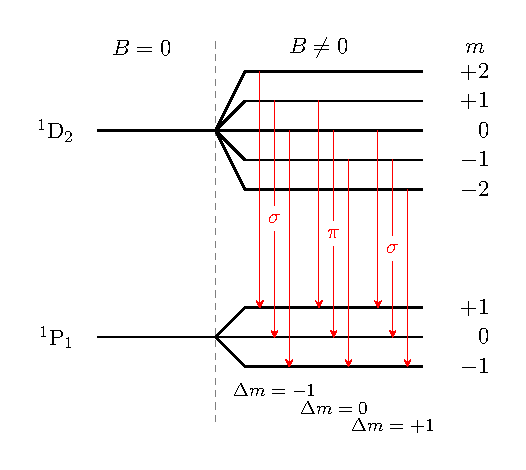
\includegraphics[scale=1.15]{../Grafiken/termschema_rot.pdf}
\caption{Hier ist das Termschema der roten Spektrallinie einer Cd-Lampe dargestellt\label{fig:termschema_rot}}
\end{figure}
\FloatBarrier
\FloatBarrier
\begin{figure}[!h]
\centering
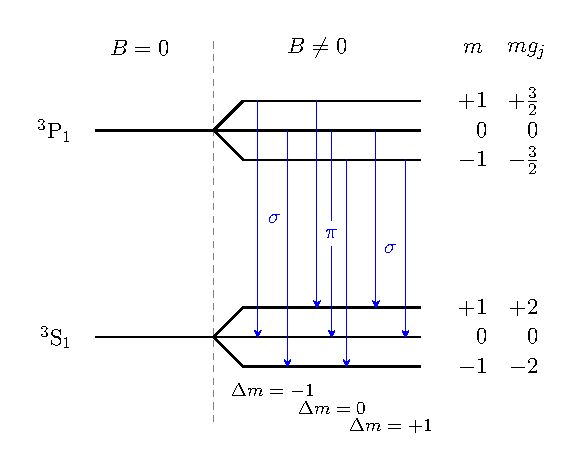
\includegraphics[scale=1.25]{../Grafiken/termschema_blau.pdf}
\caption{\label{fig:termschema_blau}}
\end{figure}
\FloatBarrier